\chapter{Daten-Kompression}
In diesem Kapitel untersuchen wir die Frage, wie wir einen gegebenen String $s$ m\"oglichst platzsparend
abspeichern k\"onnen.  Wir gehen davon aus, dass der String $s$ aus Buchstaben besteht, die 
Elemente einer Menge $\Sigma$ sind.  Die Menge $\Sigma$ bezeichnen wir als unser \emph{Alphabet}. 
Wenn das Alphabet aus $n$ verschiedenen Zeichen besteht und wir alle Buchstaben mit derselben L\"ange
von $b$ Bits kodieren wollen, dann muss f\"ur diese Zahl von Bits offenbar
\[ n \leq 2^b \] 
gelten, woraus
\[ b = \textsl{ceil}\bigl(\log_2(n)\bigr) \]
folgt.  Hier bezeichnet $\textsl{ceil}(x)$ die \emph{Ceiling-Funktion}.  Diese Funktion
rundet eine gegebene reelle Zahl immer auf, es gilt also
\[ \textsl{ceil}(x) = \min \{ k \in \N \mid x \leq k \}. \]
Besteht der String $s$ aus $m$ Buchstaben, so werden zur Kodierung des Strings insgesamt
$m \cdot b$ Bits gebraucht.  Nun gibt es zwei M\"oglichkeiten, weiterzumachen:
\begin{enumerate}
\item Lassen wir die Forderung, dass alle Buchstaben mit derselben Anzahl von Bits kodiert werden,
      fallen, dann ist es unter Umst\"anden m\"oglich, den String $s$ mit weniger Bits zu kodieren.  
      Dies f\"uhrt zu dem 1952 von David A.~Huffman angegebenen Algorithmus, den wir in den n\"achsten
      beiden Abschnitten vorstellen und analysieren.
\item Alternativ k\"onnen wir versuchen, Buchstabenkombinationen, die h\"aufig auftreten, als neue
      Buchstaben aufzufassen.  Beispielsweise kommen W\"orter wie ``\emph{der}'', ``\emph{die}'' und
      ``\emph{das}'' in deutschsprachigen Texten relativ h\"aufig vor.  Es ist daher sinnvoll, f\"ur
      solche Buchstaben-Kombinationen neue Codes einzuf\"uhren.  Ein Algorithmus, der auf dieser Idee
      basiert, ist der Lempel-Ziv-Welch Algorithmus, den wir im letzten Abschnitt dieses Kapitels 
      diskutieren werden.
\end{enumerate}


\section{Motivation des Algorithmus von Huffman}
Die zentrale Idee des von Huffman entwickelten Algorithmus ist die, dass Buchstaben, die sehr
h\"aufig auftreten, mit m\"oglichst wenig Bits kodiert werden, w\"ahrend Buchstaben, die sehr selten
auftreten, mit einer gr\"o{\ss}eren Anzahl Bits kodiert werden.  Zur Verdeutlichung betrachten
wir folgendes Beispiel:  Unser Alphabet  $\Sigma$ bestehe nur aus vier Buchstaben,
\[ \Sigma = \{ \mathtt{a}, \mathtt{b}, \mathtt{c}, \texttt{d} \}. \]
In dem zu speichernden String $s$ trete der Buchstabe \texttt{a} insgesamt $990$ mal auf, der
Buchstabe \texttt{b} trete $8$ mal auf und die Buchstaben \texttt{c} und \texttt{d} treten
jeweil $1$ mal auf.  Dann besteht der String $s$ aus insgesamt $1\,000$ 
Buchstaben.  Wenn wir jeden Buchstaben mit $2 = \log_2(4)$ Bits kodieren, dann werden also
insgesamt $2\,000$ Bits ben\"otigt um den String $s$ abzuspeichern.  Wir k\"onnen den String
aber auch mit weniger Bits abspeichern, wenn wir die einzelnen Buchstaben mit Bitfolgen
unterschiedlicher L\"ange kodieren.   In unserem konkreten
Beispiel wollen wir versuchen den Buchstaben \texttt{a}, der mit Abstand am h\"aufigsten
vorkommt, mit einem einzigen Bit zu kodieren.  Bei den  Buchstaben
\texttt{c} und \texttt{d}, die nur sehr selten auftreten, ist es kein Problem auch mehr
Bits zu verwenden.  Tabelle \ref{tab:coding} zeigt eine Kodierung, die von dieser Idee
ausgeht. 

\begin{table}[htbp]
  \centering
\begin{tabular}[t]{|l|r|r|r|r|}
\hline
Buchstabe & \texttt{a} & \texttt{b}  & \texttt{c}   & \texttt{d}   \\
\hline
Kodierung & \texttt{0} & \texttt{10} & \texttt{110} & \texttt{111} \\
\hline
\end{tabular}
  \caption{Kodierung der Buchstaben mit variabler L\"ange.}
  \label{tab:coding}
\end{table}

Um zu verstehen, wie diese Kodierung funktioniert, stellen wir sie in
Abbildung \ref{fig:coding-tree} als Baum dar.  Die inneren 
Knoten dieses Baums enthalten keine Attribute und werden als leere Kreise dargestellt.
Die Bl\"atter des Baums sind mit den Buchstaben markiert.
Die Kodierung eines Buchstabens ergibt sich \"uber die Beschriftung der Kanten, die von dem
Wurzel-Knoten zu dem Buchstaben f\"uhren.  Beispielsweise f\"uhrt von der Wurzel eine
Kante direkt zu dem Blatt, das mit dem Buchstaben ``\texttt{a}'' markiert ist.  Diese
Kante ist mit dem Label ``\texttt{0}'' beschriftet.  Also wird der Buchstabe
``\texttt{a}'' durch den String ``\texttt{0}'' kodiert.  Um ein weiteres Beispiel zu
geben, betrachten wir den Buchstaben ``\texttt{c}''.   Der Pfad, der von der Wurzel zu dem
Blatt f\"uhrt, das mit ``\texttt{c}'' markiert ist, enth\"alt drei Kanten.  Die ersten beiden
Kanten sind jeweils mit ``\texttt{1}'' markiert, die letzte Kante ist mit ``\texttt{0}''
markiert.  Also wird der Buchstabe ''\texttt{c}'' durch den String ``\texttt{110}''
kodiert.  Kodieren wir nun unseren urspr\"unglichen String $s$, der aus $990$
\texttt{a}'s, $8$ \texttt{b}'s, einem \texttt{c} und einem \texttt{d} besteht, so
ben\"otigen wir insgesamt
\[ 990 \cdot 1 + 8 \cdot 2 + 1 \cdot 3 + 1 \cdot 3 = 1\,012 \]
Bits.  Gegen\"uber der urspr\"unglichen Kodierung, die $2\,000$ Bits verwendet, haben wir $49,4\%$
gespart!

\begin{figure}[!ht]
  \centering
  \framebox{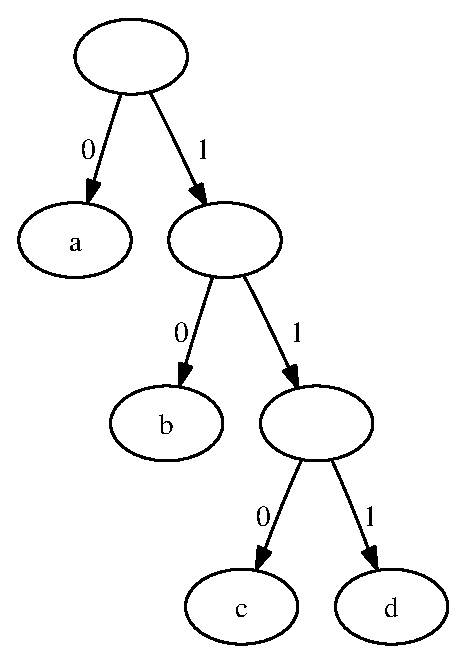
\epsfig{file=coding-tree.eps, scale=0.5}} 
  \caption{Baum-Darstellung der Kodierung.}
  \label{fig:coding-tree}
\end{figure}

Um zu sehen, wie mit Hilfe des Kodierungs-Baums ein String dekodiert werden kann,
betrachten wir als Beispiel den String ``\texttt{100111}''.  Wir beginnen mit der
``\texttt{1}'', die uns sagt, vom Wurzel-Knoten dem rechten Pfeil zu folgen.  Die
anschlie{\ss}ende ``\texttt{0}'' spezifiziert dann den linken Pfeil.  Jetzt sind wir bei dem
mit ''\texttt{b}'' markierten Blatt angekommen und haben damit den ersten Buchstaben
gefunden.  Wir gehen wieder zur Wurzel des Baums zur\"uck. Die folgende ``\texttt{0}'' f\"uhrt
uns zu dem Blatt, das mit ``\texttt{a}'' markiert ist, also haben wir den zweiten
Buchstaben gefunden. Wir gehen wieder zur Wurzel zur\"uck.  Die Ziffern ``\texttt{111}''
f\"uhren uns nun zu dem Buchstaben ``\texttt{d}''.  Damit haben wir insgesamt
\\[0.2cm]
\hspace*{1.3cm}
``\texttt{100111}'' $\simeq$ ``\texttt{bad}''.


\section{Der Algorithmus von Huffman}
Angenommen, wir haben einen String $s$, der aus Buchstaben eines Alphabets $\Sigma$
aufgebaut ist.  Wie finden wir dann eine Kodierung f\"ur die einzelnen Buchstaben, die
mit m\"oglichst wenig Bits auskommt?  Der Algorithmus von Huffman gibt eine Antwort auf diese
Frage. Um diesen Algorithmus pr\"asentieren zu k\"onnen, definieren wir die Menge
$\mathcal{K}$ der \emph{Kodierungs-B\"aume} induktiv.  
\begin{enumerate}
\item $\textsl{Leaf}(c,f) \in \mathcal{K} \quad \mbox{falls $c \in \Sigma$ und $f \in \N$}$.

      Ausdr\"ucke der Form $\textsl{Leaf}(c,f)$ sind die Bl\"atter eines Kodierungs-Baums.
      Dabei ist $c$ ein Buchstabe aus unserem Alphabet $\Sigma$ und $f$ gibt die
      H\"aufigkeit an, mit der dieser Buchstabe in dem zu kodierenden String auftritt.

      Gegen\"uber Abbildung \ref{fig:coding-tree} kommen hier bei den Bl\"attern noch die
      H\"aufigkeiten hinzu.  Diese ben\"otigen wir, denn wir wollen ja sp\"ater Buchstaben,
      die sehr h\"aufig auftreten, mit m\"oglichst wenig Bits kodieren.  

\item $\textsl{Node}(l,r) \in \mathcal{K} \quad 
       \mbox{falls $l \in\mathcal{K}$ und $r \in \mathcal{K}$.}$ 

      Ausdr\"ucke der Form $\textsl{Node}(l,r)$ sind die inneren Knoten eines
      Kodierungs-Baums.  
\end{enumerate}
Als n\"achstes  definieren wir eine Funktion 
\[  \textsl{count} : \mathcal{K} \rightarrow \N, \]
welche die  Gesamt-H\"aufigkeiten aller in dem Baum auftretenden Buchstaben aufsummiert.
\begin{enumerate}
\item Die Definition der Funktion \textsl{count} ist f\"ur Bl\"atter trivial:
      \[ \textsl{Leaf}(c,f).\textsl{count}() = f. \]
\item Die Gesamt-H\"aufigkeit des Knotens $\textsl{Node}(l,r)$
      ergibt sich als Summe der Gesamt-H\"aufigkeiten von $l$ und $r$. Also gilt
      \[ \textsl{Node}(l,r).\textsl{count}() = l.\textsl{count}() + r.\textsl{count}(). \]
\end{enumerate}
Weiter definieren wir auf Kodierungs-B\"aumen die Funktion
\[ \textsl{cost}: \mathcal{K} \rightarrow \N. \]
Die Funktion \textsl{cost} gibt an, wie viele Bits ben\"otigt werden, um mit dem gegebenen
Kodierungs-Baum eine String zu kodieren, wenn die H\"aufigkeiten, mit denen ein Buchstabe
verwendet wird, mit den H\"aufigkeiten \"ubereinstimmen, die an den Bl\"attern des Baums notiert
sind.  Die Definition dieser Funktion ist induktiv:
\begin{enumerate}
\item $\textsl{Leaf}(c,f).\textsl{cost}() = 0$,

      denn solange nur ein einziger Buchstabe vorhanden ist, ist noch nichts zu kodieren.
\item $\textsl{Node}(l,r).\textsl{cost}() = 
       l.\textsl{cost}() + r.\textsl{cost}() + l.\textsl{count}() + r.\textsl{count}()$.

      Wenn wir zwei Kodierungs-B\"aume $l$ und $r$ zu einem neuen Kodierungs-Baum
      zusammenf\"ugen, verl\"angern sich die Kodierungen f\"ur alle Buchstaben, die in $l$ oder
      $r$ auftreten, um ein Bit.
      Die Summe 
      \[ l.\textsl{count}() + r.\textsl{count}() \]
      gibt die Gesamt-H\"aufigkeiten aller Buchstaben an, die in dem linken und
      rechten Teilbaum auftreten.  Da sich die Kodierung aller dieser Buchstaben
      durch die Bildung des Knotens $\textsl{Node}(l,r)$ gegen\"uber der Kodierung in $l$
      und $r$ jeweils um 1 verl\"angert, m\"ussen wir zu den Kosten der Teilb\"aume $l$ und $r$
      den Term $l.\textsl{count}() + r.\textsl{count}()$ hinzuaddieren.
\end{enumerate}
Wir erweitern die Funktion $\textsl{cost}()$ auf Mengen von Knoten, indem wir die Kosten
einer Menge $M$ als die Summe der Kosten der Knoten von $M$ definieren:
\[ \textsl{cost}(M) = \sum\limits_{n\in M} n.\textsl{cost}(). \]
Ausgangs-Punkt des von David A.~Huffman (1925 -- 1999) im Jahre 1952 angegebenen
Algorithmus \cite{huffman:52} ist eine Menge von Paaren der Form $\langle c, f\rangle$.  Dabei ist
$c$ ein 
Buchstabe und $f$ gibt die H\"aufigkeit an, mit der dieser Buchstabe auftritt.  Im ersten
Schritt werden diese Paare in die Bl\"atter eines Kodierungs-Baums \"uberf\"uhrt.  Besteht der
zu kodierende String aus  $n$ verschiedenen Buchstaben, so haben
wir dann eine Menge von Kodierungs-B\"aumen der Form
\begin{equation}
  \label{eq:huffmann1}
 M = \bigl\{  \textsl{Leaf}(c_1, f_1), \cdots, \textsl{Leaf}(c_k, f_k) \bigr\}   
\end{equation}
Es werden nun solange Knoten $a$ und $b$ aus $M$ zu einem neuen Knoten
$\textsl{Node}(a,b)$ zusammengefasst, bis die Menge $M$ nur noch einen Knoten enth\"alt.
Offenbar gibt es im Allgemeinen sehr viele M\"oglichkeiten, die Knoten aus der Menge zu
neuen Knoten zusammen zu fassen.  Das Ziel ist es die Knoten so zusammen zu fassen, dass
die Kosten der Menge $M$ am Ende  minimal sind.
Um zu verstehen, welche Knoten wir am geschicktesten zusammenfassen k\"onnen, betrachten wir, wie
sich die Kosten der Menge durch das Zusammenfassen zweier Knoten \"andert.
Dazu betrachten wir zwei Mengen von Knoten $M_1$ und $M_2$, so dass 
\[ M_1 = N \cup \{ a, b\} \quad \mathtt{und} \quad M_2 = N \cup \{ \textsl{Node}(a,b) \} \]
gilt, die Menge $M_1$ geht also aus der Menge $M_2$ dadurch hervor, dass wir
die Knoten $a$ und $b$ zu einem neuen Knoten zusammen fassen und durch diesen ersetzen.
Untersuchen wir, wie
sich die Kosten der Menge dabei ver\"andern, wir untersuchen also die folgende Differenz:
\begin{eqnarray*}
& & \textsl{cost}\bigl(N \cup \{ \textsl{Node}(a,b) \}\bigr) - \textsl{cost}\bigl(N \cup \{ a,b \}\bigr) \\
&=& \textsl{cost}\bigl( \{ \textsl{Node}(a,b) \}\bigr) - \textsl{cost}\bigl(\{ a,b \}\bigr)              \\
&=& \textsl{Node}(a,b).\textsl{cost}() - a.\textsl{cost}() - b.\textsl{cost}()                           \\
&=&   a.\textsl{cost}() + b.\textsl{cost}() + a.\textsl{count}() + b.\textsl{count}() 
    - a.\textsl{cost}() - b.\textsl{cost}()                                                              \\
&=& a.\textsl{count}() + b.\textsl{count}() 
\end{eqnarray*}
Fassen wir die Knoten $a$ und $b$ aus der Menge $M$ zu einem neuen Knoten zusammen, so verg\"o{\ss}ern sich
die Kosten der Menge um die Summe
\[ a.\textsl{count}() + b.\textsl{count}(). \]
Wenn wir die Kosten der Menge $M$ insgesamt m\"oglichst klein halten wollen, dann ist es daher naheliegend,
dass wir in der Menge $M$ die beiden Knoten $a$ und $b$ suchen, f\"ur die die Funktion
$\textsl{count}()$ den kleinsten Wert liefert.  Diese Knoten werden wir aus der Menge $M$
entfernen und durch den neuen Knoten $\textsl{Node}(a,b)$ ersetzen.
Dieser Prozess wird solange iteriert, bis die Menge $M$ nur noch aus einem Knoten besteht.  Dieser
Knoten ist dann die Wurzel des gesuchten Kodierungs-Baums. 

\begin{figure}[!ht]
\centering
\begin{Verbatim}[ frame         = lines, 
                  framesep      = 0.3cm, 
                  labelposition = bottomline,
                  numbers       = left,
                  numbersep     = -0.2cm,
                  xleftmargin   = 1.3cm,
                  xrightmargin  = 1.3cm,
                ]
    codingTree := procedure(m) {
        while (#m > 1) {
            a := first(m);
            m -= { a };
            b := first(m);
            m -= { b };
            m += { [ count(a) + count(b), Node(a, b) ] };
        }
        return arb(m);
    };    
    count := p |-> p[1];
\end{Verbatim}
\vspace*{-0.3cm}
\caption{Der Algorithmus von Huffman in \textsc{SetlX}.}
\label{fig:huffman.stlx}
\end{figure} % $

\noindent
Die in Abbildung \ref{fig:huffman.stlx} gezeigte Funktion $\mathtt{codingTree}(m)$
implementiert diesen Algorithmus. 
\begin{enumerate}
\item Die Funktion \textsl{codingTree} wird mit einer Menge $m$ von Knoten aufgerufen,
      welche die Form
      \\[0.2cm]
      \hspace*{1.3cm}
      $m = \bigl\{ \langle f_1, \textsl{Leaf}(c_1) \rangle, \cdots, 
                  \langle f_k, \textsl{Leaf}(c_k) \rangle \bigr\}   
      $
      \\[0.2cm]
      hat.  Hier bezeichnen die Variablen $c_i$ die verschiedenen Buchstaben, w\"ahrend die
      Zahl $f_i$ die H\"aufigkeit angibt, mit der der Buchstabe $c_i$ auftritt.

      Wir haben hier die Information \"uber die H\"aufigkeit an erster Stelle eines Paares gespeichert.
      Da \textsc{SetlX} diese Menge intern durch einen geordneten bin\"aren Baum
      abspeichert, erm\"oglicht uns diese Form der Darstellung einfach auf den Knoten mit
      der kleinsten H\"aufigkeit zuzugreifen, denn die Paare werden so verglichen, dass
      immer zun\"achst die erste Komponente zweier Paare zum Vergleich herangezogen werden.
      Nur wenn sich in der ersten Komponente kein Unterschied ergibt, wird auch die zweite
      Komponente verglichen.  Daher finden wir das Paar mit der kleinsten ersten
      Komponente immer am Anfang der Menge $m$.

      Durch diesen Trick haben wir uns de facto die Implementierung einer
      Priorit\"ats-Warteschlange gespart:  
      \begin{enumerate}
      \item Die in \textsc{SetlX} vordefinierte Funktion
            $\mathtt{first}(m)$ liefert das erste Element der Menge $m$ und entspricht
            damit der Funktion $\textsl{top}(m)$ des abstrakten Daten-Typs \textsl{PrioQueue}.
      \item Anstelle von $\textsl{insert}(m, p, v)$ k\"onnen wir einfach
            \\[0.2cm]
            \hspace*{1.3cm}
            \texttt{$m$ += \{ [$p$, $v$] \};}
            \\[0.2cm]
            schreiben um das Element $v$ mit der Priorit\"at $p$ in die
            Priorit\"ats-Warteschlange $m$ einzuf\"ugen.
      \item Die Funktion $\textsl{remove}(m)$ realisieren wir durch den Aufruf
            \\[0.2cm]
            \hspace*{1.3cm}
            \texttt{$m$ -= \{ first($m$) \};}
            \\[0.2cm]
            denn $\textsl{remove}(m)$ soll ja das Element mit der h\"ochsten Priorit\"at aus
            $m$ entfernen.
      \end{enumerate}
      Das Elegante an diesem Vorgehen ist, dass damit s\"amtliche Operationen des abstrakten
      Daten-Typs \textsl{PrioQueue} eine logarithmische Komplexit\"at haben.  Das ist zwar
      im Falle der Operation $\textsl{top}(m)$ nicht optimal, aber f\"ur die Praxis v\"ollig
      ausreichend, denn in der Praxis kommt auf jeden Aufruf der Form $\textsl{top}(m)$
      auch ein Aufruf der Form $\textsl{remove}(m)$ und der hat sowohl bei einer optimalen
      Implementierung als auch bei unserer Implementierung eine logarithmische
      Komplexit\"at, die dann auch im Falle der optimalen Implementierung  die gesamte
      Komplexit\"at dominiert. 
\item Die \texttt{while}-Schleife in Zeile 2 veringert die Anzahl der Knoten in der Menge $m$
      in jedem Schritt um Eins.  
      \begin{enumerate}
      \item Dazu werden mit Hilfe der Funktion $\textsl{first}()$ die
            beiden Knoten $a$ und $b$ berechnet, f\"ur die der Wert von $\textsl{count}()$ minimal
            ist.  Die Funktion $\mathtt{count}(p)$ ist in Zeile 11 definiert und liefert einfach die
            erste Komponente des Paares $p$, denn dort speichern wir die H\"aufigkeit der Buchstaben 
            ab.
      \item Die beiden Knoten $a$ und $b$ mit der geringsten H\"aufigkeit werden in Zeile 4 und 6
            aus der Menge $m$ entfernt.
      \item Anschlie{\ss}end wird aus den beiden Knoten $a$ und $b$ ein neuer Knoten 
            $\textsl{Node}(a,b)$ gebildet.
            Dieser neue Knoten wird zusammen mit der Gesamth\"aufigkeit der Knoten $a$ und $b$ in Zeile
            7 der Menge $m$ hinzugef\"ugt.
      \end{enumerate}
\item Die \texttt{while}-Schleife wird beendet, wenn die Menge $m$ nur noch ein Element enth\"alt.
      Dieses wird mit der Funktion \texttt{arb} extrahiert und als Ergebnis zur\"uck gegeben.
\end{enumerate}
Die Laufzeit des Huffman-Algorithmus h\"angt stark von der Effizienz der Funktion $\textsl{first}()$ ab.
Eine naive Implementierung w\"urde die Knoten aus der Menge $m$ in einer geordneten Liste vorhalten.
Die Knoten $n$ w\"aren in dieser Liste nach der Gr\"o{\ss}e $n.\textsl{cost}()$ aufsteigend sortiert.
Dann ist die Funktion $\textsl{first}()$ zwar sehr effizient, aber das Einf\"ugen des neuen Knotens,
dass wir oben \"uber den Befehl 
\\[0.2cm]
\hspace*{1.3cm}
\texttt{m += \{ [ count(a) + count(b), Node(a, b) ] \};}
\\[0.2cm]
realisieren,  w\"urde einen Aufwand erfordern, der linear in der Anzahl der Elemente der Menge $m$ ist.
Dadurch, dass wir mit einer Menge  $m$ arbeiten, die in \textsc{SetlX} intern durch einen
Rot-Schwarz-Baum dargestellt ist, erreichen wir, dass alle in der \texttt{while}-Schleife durchgef\"uhrten
Operationen nur logarithmisch von der Anzahl der Buchstaben abh\"angen.  Damit hat der Huffman-Algorithmus
insgesamt die Komplexit\"at $\Oh\bigl(n \cdot \ln(n)\bigr)$.
 

\begin{table}[htbp]
  \centering
\begin{tabular}[t]{|l|r|r|r|r|r|}
\hline
Buchstabe  & \texttt{a} & \texttt{b} & \texttt{c} & \texttt{d} & \texttt{e} \\
\hline
H\"aufigkeit &          1 &          2 &          3 &          4 &          5 \\
\hline
\end{tabular}
  \caption{Buchstaben mit H\"aufigkeiten.}
  \label{tab:frequency}
\end{table}

Wir illustrieren den  Huffman-Algorithmus, indem wir ihn auf die Buchstaben, die in
Tabelle \ref{tab:frequency} zusammen mit ihren H\"aufigkeiten angegeben sind, anwenden.
\begin{enumerate}
\item Zu Beginn hat die Menge $m$ die Form
      \\[0.2cm]
      \hspace*{1.3cm}
      $ m = \bigl\{ \langle 1, \textsl{Leaf}(\mathtt{a}) \rangle,\,
             \langle 2, \textsl{Leaf}(\mathtt{b}) \rangle,\, 
             \langle 3, \textsl{Leaf}(\mathtt{c}) \rangle,\,
             \langle 4, \textsl{Leaf}(\mathtt{d}) \rangle,\,
             \langle 5, \textsl{Leaf}(\mathtt{e}) \rangle\bigr\}. $
\item Die H\"aufigkeit ist hier f\"ur die Bl\"atter mit den Buchstaben \texttt{a} und
      \texttt{b} minimal.  Also entfernen wir diese Bl\"atter aus der Menge und f\"ugen statt
      dessen den Knoten 
      \\[0.2cm]
      \hspace*{1.3cm}
      $\textsl{Node}(\textsl{Leaf}(\mathtt{a}), \textsl{Leaf}(\mathtt{b}))$
      \\[0.2cm]
      in die Menge $m$ ein.  Die H\"aufigkeit dieses Knotens ergibt sich als Summe der H\"aufigkeiten
      der Buchstaben \texttt{a} und \texttt{b}. Daher f\"ugen wir insgesamt das Paar
      \\[0.2cm]
      \hspace*{1.3cm}
      $\langle 3, \textsl{Node}\bigl(\textsl{Leaf}(\mathtt{a}) \rangle, \textsl{Leaf}(\mathtt{b}) \bigr) \rangle$
      \\[0.2cm]
      in die Menge $m$ ein.        Dann hat $m$ die Form
      \\[0.2cm]
      \hspace*{1.3cm}
      $ \bigl\{\langle 3, \textsl{Node}(\textsl{Leaf}(\mathtt{a}), \textsl{Leaf}(\mathtt{b}))\rangle,\,
             \langle 3, \textsl{Leaf}(\mathtt{c}) \rangle,\, \langle 4, \textsl{Leaf}(\mathtt{d}) \rangle,\,
             \langle 5, \textsl{Leaf}(\mathtt{e}) \rangle\bigr\}. $
\item Die beiden Paare mit den kleinsten Werten der H\"aufigkeiten in $m$ sind nun
      \\[0.2cm]
      \hspace*{1.3cm}
      $ \langle 3, \textsl{Node}(\textsl{Leaf}(\mathtt{a}), \textsl{Leaf}(\mathtt{b})) \rangle
         \quad \mathrm{und} \quad \langle 3, \textsl{Leaf}(\mathtt{c})\rangle$.
      \\[0.2cm]
      Wir entfernen diese beiden Knoten und bilden aus diesen beiden Knoten den neuen Knoten
      \\[0.2cm]
      \hspace*{1.3cm}
      $ \langle 6, \textsl{Node}(
           \textsl{Node}((\textsl{Leaf}(\mathtt{a}), \textsl{Leaf}(\mathtt{b})),\; 
           \textsl{Leaf}(\mathtt{c}))\rangle, $
      \\[0.2cm]
      den wir der Menge $m$ hinzuf\"ugen.  Dann hat $m$ die Form
      \\[0.2cm]
      \hspace*{1.3cm}
      $ \Bigl\{ 
        \langle 4, \textsl{Leaf}(\mathtt{d}) \rangle,\;\langle 5, \textsl{Leaf}(\mathtt{e}) \rangle,\;
        \langle 6, \textsl{Node}(
           \textsl{Node}(\textsl{Leaf}(\mathtt{a}), \textsl{Leaf}(\mathtt{b})),\; 
           \textsl{Leaf}(\mathtt{c}))\Bigr\}. $
\item Jetzt sind 
      \\[0.2cm]
      \hspace*{1.3cm}
      $ \langle 4, \textsl{Leaf}(\mathtt{d}) \rangle \quad \mathrm{und} \quad \langle 5, \textsl{Leaf}(\mathtt{e}) \rangle$
      \\[0.2cm]
      die beiden Knoten mit dem kleinsten Werten der H\"aufigkeit.
      Wir entfernen diese Knoten und bilden den neuen Knoten \\[0.2cm]
      \hspace*{1.3cm}
      $\langle 9, \textsl{Node}(\textsl{Leaf}(\mathtt{d}), \textsl{Leaf}(\mathtt{e})) \rangle$.
      \\[0.2cm]
      Diesen f\"ugen wir der Menge $m$ hinzu und erhalten
      \\[0.2cm]
      \hspace*{1.3cm}
      $ \Bigl\{ 
        \langle 6, \textsl{Node}(
           \textsl{Node}(\textsl{Leaf}(\mathtt{a}),
           \textsl{Leaf}(\mathtt{b})),\,\textsl{Leaf}(\mathtt{c},3))
        \rangle,\;
        \langle 9,\textsl{Node}(\textsl{Leaf}(\mathtt{d},4), \textsl{Leaf}(\mathtt{e},5)) \rangle
        \Bigr\}
           $.      
\item Jetzt enth\"alt die Menge $m$ nur noch zwei Knoten.  Wir entfernen diese beiden Knoten und
      bilden daraus den neuen Knoten
      \\[0.2cm]
      \hspace*{1.3cm}
      $\textsl{Node}\biggl(
              \textsl{Node}\Bigl(
                 \textsl{Node}\bigl(\textsl{Leaf}(\mathtt{a}), \textsl{Leaf}(\mathtt{b})\bigr),\; 
                 \textsl{Leaf}(\mathtt{c})\Bigr),\;
              \textsl{Node}\bigl(\textsl{Leaf}(\mathtt{d}), \textsl{Leaf}(\mathtt{e})\bigr)
         \biggr)
      $
      \\[0.2cm]
      Dieser Knoten ist jetzt der einzige Knoten in $m$ und damit unser Ergebnis.
      Stellen wir diesen Knoten als Baum dar, so erhalten wir das in Abbildung
      \ref{fig:coding-tree2} gezeigte Ergebnis.  Wir haben hier jeden Knoten $n$
      mit dem Funktionswert  $n.\textsl{count}()$ beschriftet.  

      Die Kodierung, die sich daraus ergibt,
      wird in Tabelle \ref{tab:coding2} gezeigt.
\end{enumerate}

\begin{figure}[!ht]
  \centering
  \framebox{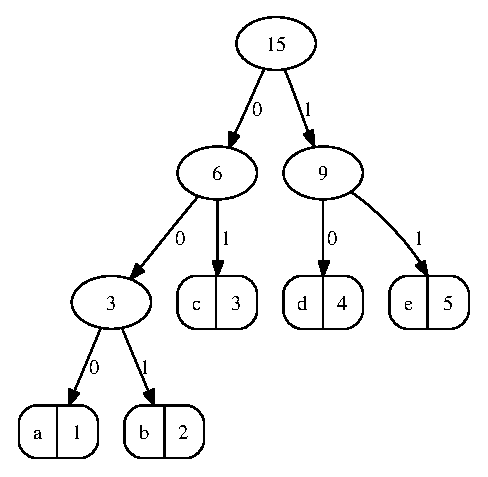
\epsfig{file=coding-tree2.eps, scale=0.7}} 
  \caption{Baum-Darstellung der Kodierung.}
  \label{fig:coding-tree2}
\end{figure}



\begin{table}[htbp]
  \centering
\begin{tabular}[t]{|l|r|r|r|r|r|}
\hline
Buchstabe &   \texttt{a} &   \texttt{b} & \texttt{c}  & \texttt{d}  & \texttt{e}   \\
\hline
Kodierung & \texttt{000} & \texttt{001} & \texttt{01} & \texttt{10} & \texttt{11} \\
\hline
\end{tabular}
  \caption{Kodierung der Buchstaben mit variabler L\"ange.}
  \label{tab:coding2}
\end{table}


\exercise
\begin{enumerate}
\item Berechnen Sie den Huffman-Code f\"ur einen Text, der nur die Buchstaben
      ``\texttt{a}'' bis ``\texttt{g}'' enth\"alt und f\"ur den die H\"aufigkeiten,
      mit denen diese Buchstaben auftreten, durch die folgende Tabelle gegeben sind.

\begin{table}[htbp]
  \centering
\begin{tabular}[t]{|l|r|r|r|r|r|r|r|}
\hline
Buchstabe  & \texttt{a} & \texttt{b} & \texttt{c} & \texttt{d} & \texttt{e} & \texttt{f} & \texttt{g} \\
\hline
H\"aufigkeit &          1 &          1 &          2 &          3 &          5 &         8 &         13 \\
\hline
\end{tabular}
  \caption{Buchstaben mit H\"aufigkeiten.}
  \label{tab:aufgabe-huffman}
\end{table}

\item Wie gro{\ss} ist die Einsparung, wenn man die Buchstaben mit einem Huffman-Code
      kodiert gegen\"uber einer Kodierung mit drei Bits?
\item Versuchen Sie das Gesetz zu erkennen, nach dem die H\"aufigkeiten in der obigen Tabelle 
      gebildet wurden und versuchen Sie, den Huffman-Code f\"ur den allgemeinen Fall,
      in dem $n$ Buchstaben gegeben sind, anzugeben.
\item Wie gro{\ss} ist die Einsparung im allgemeinen Fall?
\end{enumerate}

\section{Optimalit\"at des Huffman'schen Kodierungsbaums}
In diesem Abschnitt zeigen wir, dass der durch den Algorithmus von Huffman berechnete Kodie\-rungs-Baum der
Kodierungs-Baum ist, f\"ur den die Funktion $\textsl{cost}()$ minimal ist.  Dazu geben zun\"achst eine andere
Formel zur Berechnung von $n.\textsl{cost}()$ an:  Wir definieren die \emph{Tiefe}
$n.\textsl{depth}(c)$ des Buchstabens $c$ in dem Kodierungs-Baum $n$ als den Abstand, den das Blatt $l$,
das mit dem Buchstaben $c$ markiert ist, von der Wurzel des Kodierungs-Baums hat.  Der Kodierungs-Baum
wird dabei als Graph aufgefasst.  Dann gibt es genau einen Pfad von der Wurzel zu dem Blatt $l$ und 
$n.\textsl{depth}(c)$ wird als die Anzahl der Kanten dieses Pfades definiert.
Jede der Kanten dieses Pfades tr\"agt hinterher ein Bit zur 
Kodierung des Buchstabens bei, mit dem das Blatt $l$ markiert ist.  Um die gesamten Kosten zu berechnen
m\"ussen wir daher die Tiefe jedes Buchstabens mit seiner H\"aufigkeit multiplizieren.  Bezeichnen wir die
H\"aufigkeit des Buchstabens $c$ mit $\textsl{freq}(c)$, so erhalten wir insgesamt
\begin{equation}
  \label{eq:cost}
  n.\textsl{cost}() = \sum\limits_{c\in\Sigma} \textsl{freq}(c) \cdot n.\textsl{depth}(c)
\end{equation}
Die Summe l\"auft dabei \"uber alle Buchstaben des Alphabets $\Sigma$, wobei wir voraussetzen,
dass alle Buchstaben aus $\Sigma$ auch tats\"achlich in dem Kodierungs-Baum auftreten.
Buchstaben, die gar nicht auftreten, werden also vorher aus dem Alphabet entfernt.

\begin{Definition}[Optimaler Kodierungs-Baum]
  Ein Kodierungs-Baum $n$ ist \emph{optimal}, wenn bei gegebener H\"aufigkeit der Buchstaben
  der Wert $n.\textsl{cost}()$ minimal ist, f\"ur alle Kodierungs-B\"aume $k$, bei denen die
  Buchstaben mit derselben H\"aufigkeit auftreten wie in $n$,  gilt also
  \\[0.2cm]
  \hspace*{1.3cm} $n.\textsl{cost}() \leq k.\textsl{cost}()$.
\end{Definition}


\begin{Lemma}
  \label{huffman:l1}
  Es seien $x$ und $y$ die beiden Buchstaben aus dem Alphabet $\Sigma$ mit der geringsten H\"aufigkeit.  Dann
  gibt es einen optimalen Kodierungs-Baum $n$, bei dem sich die Kodierung der Buchstaben $x$ und $y$ nur im
  letzten Bit unterscheidet.
\end{Lemma}

\noindent
\textbf{Beweis}:  Es sei $n_1$ ein optimaler Kodierungs-Baum.  Wir zeigen, wie $n_1$ zu einem
Kodierungs-Baum $n_2$ umgebaut werden kann, der einerseits optimal ist und bei dem sich andererseits die
Kodierung der Buchstaben $x$ und $y$ nur im letzten Bit unterscheidet.  Wir suchen in dem Kodierungs-Baum
$n_1$ einen Knoten $k$ der Form $\textsl{Node}(l,r)$, der unter allen \emph{inneren} Knoten eine maximale
Tiefe hat.  Dabei bezeichnen wir alle Knoten, die keine Bl\"atter sind, als innere Knoten.
An dem Knoten $k$ h\"angen zwei Buchstaben $a$ und $b$.  Wir machen nun o.B.d.A.~die folgenden Annahmen
\"uber die H\"aufigkeiten der Buchstaben:
\begin{enumerate}
\item $\textsl{freq}(x) \leq \textsl{freq}(y)$,
\item $\textsl{freq}(a) \leq \textsl{freq}(b)$.
\end{enumerate}
Da wir angenommen haben, dass $x$ und $y$ die Buchstaben mit der geringsten H\"aufigkeiten sind, folgt
daraus
\begin{equation}
  \label{eq:huffmannL0}
\textsl{freq}(x) \leq \textsl{freq}(a) \quad \textrm{und} \quad 
\textsl{freq}(y) \leq \textsl{freq}(b).  
\end{equation}
Wir erhalten nun den Kodierungs-Baum $n_2$ aus dem Kodierungs-Baum $n_1$, indem wir in dem Baum $n_1$ die
Positionen der Buchstaben $x$ und $a$ und die Positionen der Buchstaben $y$ und $b$ vertauschen.
Daher gilt 
  \begin{eqnarray}
    \label{eq:huffmannL1a}
 n_2.\textsl{depth}(a) &=& n_1.\textsl{depth}(x), \\
    \label{eq:huffmannL1b}
 n_2.\textsl{depth}(b) &=& n_1.\textsl{depth}(y), \\
    \label{eq:huffmannL1c}
 n_2.\textsl{depth}(x) &=& n_1.\textsl{depth}(a), \\
    \label{eq:huffmannL1d}
 n_2.\textsl{depth}(y) &=& n_1.\textsl{depth}(b).
  \end{eqnarray}
denn $a$ und $x$ und $b$ und $y$ vertauschen die Pl\"atze.  F\"ur alle Buchstaben
$c \in \Sigma\backslash\{a,b,x,y\}$ gilt nat\"urlich 
\begin{equation}
  \label{eq:huffmannL1e}
n_2.\textsl{depth}(c) = n_1.\textsl{depth}(c).   
\end{equation}
Weiterhin wissen wir aufgrund der Auswahl des Knotens $k$, dass
\begin{eqnarray}
  \label{eq:huffmannL2a}
  n_1.\textsl{depth}(a) = n_1.\textsl{depth}(b) \geq n_1.\textsl{depth}(x) \quad \mathrm{und} \\
  \label{eq:huffmannL2b}
  n_1.\textsl{depth}(a) = n_1.\textsl{depth}(b) \geq n_1.\textsl{depth}(y) \hspace*{0.95cm}
\end{eqnarray}
gilt.  Wir zeigen nun, dass $n_2.\textsl{cost}() \leq n_1.\textsl{cost}()$ gilt.  Dazu geben wir zun\"achst
$n_2.\textsl{cost}()$ an.
\begin{eqnarray*}
  n_2.\textsl{cost}() 
  & = & \sum\limits_{c\in\Sigma} \textsl{freq}(c) \cdot n_2.\textsl{depth}(c) \\
  & = & \sum\limits_{c\in\Sigma\backslash\{a,b,x,y\}} \textsl{freq}(c) \cdot n_2.\textsl{depth}(c) \\[0.3cm]
  &   & + \;\textsl{freq}(a) \cdot n_2.\textsl{depth}(a) 
        + \textsl{freq}(b) \cdot n_2.\textsl{depth}(b) \\[0.1cm]
  &   & + \;\textsl{freq}(x) \cdot n_2.\textsl{depth}(x) 
        + \textsl{freq}(y) \cdot n_2.\textsl{depth}(y) 
\end{eqnarray*}
Unter Ber\"ucksichtigung der Gleichungen (\ref{eq:huffmannL1a}) bis (\ref{eq:huffmannL1e}) k\"onnen wir dies
auch schreiben als
\begin{eqnarray*}  
  n_2.\textsl{cost}() 
  & = & \sum\limits_{c\in\Sigma\backslash\{a,b,x,y\}} \textsl{freq}(c) \cdot n_1.\textsl{depth}(c) \\[0.3cm]
  &   & + \;\textsl{freq}(a) \cdot n_1.\textsl{depth}(x) 
        + \textsl{freq}(b) \cdot n_1.\textsl{depth}(y) \\[0.1cm]
  &   & + \;\textsl{freq}(x) \cdot n_1.\textsl{depth}(a) 
        + \textsl{freq}(y) \cdot n_1.\textsl{depth}(b) 
\end{eqnarray*}
Analog berechnen wir $n_1.\textsl{cost}()$:
\begin{eqnarray*}
  n_1.\textsl{cost}() 
  & = & \sum\limits_{c\in\Sigma} \textsl{freq}(c) \cdot n_1.\textsl{depth}(c) \\
  & = & \sum\limits_{c\in\Sigma\backslash\{a,b,x,y\}} \textsl{freq}(c) \cdot n_1.\textsl{depth}(c) \\[0.3cm]
  &   & + \;\textsl{freq}(a) \cdot n_1.\textsl{depth}(a) 
        + \textsl{freq}(b) \cdot n_1.\textsl{depth}(b) \\[0.1cm]
  &   & + \;\textsl{freq}(x) \cdot n_1.\textsl{depth}(x) 
        + \textsl{freq}(y) \cdot n_1.\textsl{depth}(y) 
\end{eqnarray*}
Damit sehen wir, dass $n_2.\textsl{cost}() \leq n_1.\textsl{cost}()$ genau dann gilt, wenn die
Ungleichung 
\\[0.2cm]
\hspace*{-0.3cm}
$\textsl{freq}(a) \cdot n_1.\textsl{depth}(x) 
      + \textsl{freq}(b) \cdot n_1.\textsl{depth}(y) 
      + \textsl{freq}(x) \cdot n_1.\textsl{depth}(a) 
      + \textsl{freq}(y) \cdot n_1.\textsl{depth}(b)$ \\[0.1cm]
\hspace*{-0.8cm}
$\leq\; \textsl{freq}(a) \cdot n_1.\textsl{depth}(a) 
      + \textsl{freq}(b) \cdot n_1.\textsl{depth}(b) 
      + \textsl{freq}(x) \cdot n_1.\textsl{depth}(x) 
      + \textsl{freq}(y) \cdot n_1.\textsl{depth}(y)$ \\[0.2cm]
erf\"ullt ist.  Da in dieser Ungleichung nur noch der Kodierungs-Baum $n_1$ vorkommt, vereinfachen wir die
Schreibweise und vereinbaren, dass wir einen Ausdruck der Form $n_1.\textsl{depth}(u)$ zu
$\textsl{depth}(u)$ abk\"urzen.  Die letzte Ungleichung ist dann \"aquivalent zu der Ungleichung
\\[0.2cm]
\hspace*{0.8cm}
$0 \;\leq\; \textsl{freq}(a) \cdot \bigl(\textsl{depth}(a) - \textsl{depth}(x)\bigr)
          + \textsl{freq}(b) \cdot \bigl(\textsl{depth}(b) - \textsl{depth}(y)\bigr)$ 
\\[0.2cm]
\hspace*{1.3cm}
$        -\;\textsl{freq}(x) \cdot \bigl(\textsl{depth}(a) - \textsl{depth}(x)\bigr) 
         - \textsl{freq}(y) \cdot \bigl(\textsl{depth}(b) - \textsl{depth}(y)\bigr)$ \\[0.2cm]
Diese Ungleichung vereinfachen wir zu 
\\[0.3cm]
\hspace*{-0.8cm}
$0 \;\leq\; 
  \underbrace{\bigl(\textsl{freq}(a) - \textsl{freq}(x)\bigr)}_{\geq 0}   \cdot 
  \underbrace{\bigl(\textsl{depth}(a) - \textsl{depth}(x)\bigr)}_{\geq 0}
+ \underbrace{\bigl(\textsl{freq}(b) - \textsl{freq}(y)\bigr)}_{\geq 0}   \cdot 
  \underbrace{\bigl(\textsl{depth}(b) - \textsl{depth}(y)\bigr)}_{\geq 0}$
\\[0.3cm]
Hier gilt $\textsl{freq}(a) - \textsl{freq}(x) \geq 0$ wegen Ungleichung \ref{eq:huffmannL0},
die Ungleichung
\\[0.2cm]
\hspace*{1.3cm}
 $\textsl{depth}(a) - \textsl{depth}(x) \geq 0$ 
\\[0.2cm] 
folgt aus Ungleichung \ref{eq:huffmannL2a},
die Ungleichung $\textsl{freq}(b) - \textsl{freq}(y) \geq 0$ folgt aus Un\-glei\-chung \ref{eq:huffmannL0}
und die Ungleichung $\textsl{depth}(b) - \textsl{depth}(y) \geq 0$ 
folgt aus Ungleichung \ref{eq:huffmannL2b}.
Damit haben wir 
\[ n_2.\textsl{cost}() \leq n_1.\textsl{cost}() \]
gezeigt.  Da $n_1$ optimal ist, muss auch $n_2$ optimal sein.  Nach Wahl des Knotens $k$ unterscheiden
sich die Kodierungen von $x$ und $y$ nur in dem letzten Bit. Damit ist $n_2$ der gesuchte
Kodierungs-Baum.
\hspace*{\fill} $\Box$

\begin{Proposition}
  Der Kodierungs-Baum, der von dem Huffman-Algorithmus erzeugt wird, ist optimal.
\end{Proposition}

\noindent
\textbf{Beweis}:  Wir beweisen den Satz durch Induktion \"uber die Anzahl $n$ der Buchstaben in dem
Alphabet $\Sigma$.
\begin{enumerate}
\item[I.A.:] $n = 2$.  Es sei $\Sigma= \{a,b\}$.
  In diesem Fall f\"uhrt der Huffman-Algorithmus nur einen Schritt durch und liefert den Kodierungs-Baum 
  \\[0.2cm]
  \hspace*{1.3cm}
  $k=\textsl{Node}\bigl(\textsl{Leaf}(a, \textsl{freq}(a)), \textsl{Leaf}(b,\textsl{freq}(b))\bigr)$.
  \\[0.2cm]
  Bei der Kodierung eines Alphabets, das aus zwei Buchstaben besteht, haben wir keine Wahl, 
  was die L\"ange der Kodes angeht: Wir brauchen f\"ur jeden Buchstaben genau ein Bit und daher ist das vom
  Huffman-Algorithmus in diesem Fall gelieferte Ergebnis offenbar optimal.
\item[I.S.:] $n \mapsto n+1$

  Wir gehen jetzt davon aus, dass das Alphabet $\Sigma$ aus $n+1$ Buchstaben besteht.
  Es seien $x$ und $y$ die beiden Buchstaben, deren H\"aufigkeit minimal ist.
  Es sei $z$ ein neuer Buchstabe, der nicht in dem Alphabet $\Sigma$ auftritt.  Wir definieren
  ein neues Alphabet $\Sigma'$ als
  \\[0.2cm]
  \hspace*{1.3cm}
  $\Sigma' = \bigl(\Sigma \backslash \{x,y\}\bigr) \cup \{z\}$.
  \\[0.2cm]
  Die H\"aufigkeit des neuen Buchstabens $z$ definieren wir als 
  \\[0.2cm]
  \hspace*{1.3cm}
  $\textsl{freq}(z) := \textsl{freq}(x) + \textsl{freq}(y)$.
  \\[0.2cm]
  Dann enth\"alt das Alphabet $\Sigma'$ insgesamt $n$ Buchstaben.  Wenden wir den Huffman-Algorithmus
  auf dieses Alphabet an, so erhalten wir nach Induktions-Voraussetzung f\"ur $\Sigma'$ einen optimalen
  Kodierungs-Baum $k_1$.  Die Anwendung des Huffman-Algorithmus auf das Alphabet $\Sigma$ ersetzt in diesem
  Kodierungs-Baum das Blatt, das mit dem Buchstaben $z$ markiert ist, durch den Knoten 
  \\[0.2cm]
  \hspace*{1.3cm}
  $\textsl{Node}\bigl(\textsl{Leaf}(x, \textsl{freq}(x)), \textsl{Leaf}(y,\textsl{freq}(y))\bigr)$.
  \\[0.2cm]
  Bezeichnen wir den so entstanden Kodierungs-Baum mit $k_2$, so m\"ussen wir zeigen, dass $k_2$ optimal
  ist.  Wir f\"uhren den Beweis indirekt und nehmen an, dass $k_2$ nicht optimal ist. Dann gibt es einen
  Kodierungs-Baum $k_3$ f\"ur das Alphabet $\Sigma$, so dass 
  \\[0.2cm]
  \hspace*{1.3cm}
  $k_3.\textsl{cost}() < k_2.\textsl{cost}()$
  \\[0.2cm]
  ist.  Nach Lemma \ref{huffman:l1} k\"onnen wir o.B.d.A. voraussetzen, dass sich die Kodierung der 
  Buchstaben $x$ und $y$ in dem Kodierungs-Baum $k_3$ nur in dem letzten Bit
  unterscheidet.  Also gibt es in dem Kodierungs-Baum $k_3$ einen Knoten der Form
  \\[0.2cm]
  \hspace*{1.3cm}
  $\textsl{Node}\bigl(\textsl{Leaf}(x, \textsl{freq}(x)), \textsl{Leaf}(y,\textsl{freq}(y))\bigr)$.
  \\[0.2cm]
  Wir transformieren den Kodierungs-Baum $k_3$ in einen Kodierungs-Baum $k_4$ f\"ur das Alphabet $\Sigma'$ indem
  wir diesen Knoten durch das Blatt
  \\[0.2cm]
  \hspace*{1.3cm}
  $\textsl{Leaf}\bigl(z, \textsl{freq}(x) + \textsl{freq}(y)\bigr)$
  \\[0.2cm]
  ersetzen.  Damit gilt
  \begin{eqnarray*}
      k_4.\textsl{cost}() 
  &=& \sum\limits_{c\in\Sigma'} \textsl{freq}(c) \cdot k_4.\textsl{depth}(c) \\[0.3cm]
  &=& \sum\limits_{c\in\Sigma\backslash\{x,y\}\cup\{z\}} \textsl{freq}(c) \cdot k_4.\textsl{depth}(c) 
      \\[0.3cm]
  &=& \sum\limits_{c\in\Sigma\backslash\{x,y\}} \textsl{freq}(c) \cdot k_4.\textsl{depth}(c) 
      +\textsl{freq}(z) \cdot k_4.\textsl{depth}(z) \\[0.3cm]  
  &=& \sum\limits_{c\in\Sigma\backslash\{x,y\}} \textsl{freq}(c) \cdot k_3.\textsl{depth}(c) 
      +\textsl{freq}(z) \cdot \bigl(k_3.\textsl{depth}(x) - 1\bigr) \\[0.3cm]  
  &=& \sum\limits_{c\in\Sigma\backslash\{x,y\}} \textsl{freq}(c) \cdot k_3.\textsl{depth}(c) \\[0.3cm]
  & & +\; \bigl(\textsl{freq}(x) + \textsl{freq}(y)\bigr) \cdot \bigl(k_3.\textsl{depth}(x) - 1\bigr) 
      \\[0.3cm]  
  &=& \sum\limits_{c\in\Sigma} \textsl{freq}(c) \cdot k_3.\textsl{depth}(c) -\; \bigl(\textsl{freq}(x) + \textsl{freq}(y)\bigr)  
      \\[0.3cm]  
  &=& k_3.\textsl{cost}() - \bigl(\textsl{freq}(x) + \textsl{freq}(y)\bigr)  
  \end{eqnarray*}
  Wir halten dieses Ergebnis in einer Gleichung fest:
  \begin{equation}
    \label{eq:huffmanns1}
    k_4.\textsl{cost}() = k_3.\textsl{cost}() - \bigl(\textsl{freq}(x) + \textsl{freq}(y)\bigr).
  \end{equation}
  Da die Kodierungs-B\"aume $k_1$ und $k_2$ in derselben Relation stehen wie die Kodierungs-B\"aume
  $k_4$ und $k_3$, gilt analog
  \begin{equation}
    \label{eq:huffmanns2}
    k_1.\textsl{cost}() = k_2.\textsl{cost}() - \bigl(\textsl{freq}(x) + \textsl{freq}(y)\bigr). 
  \end{equation}
  Damit k\"onnen wir zeigen, dass die Kosten des Kodierungs-Baums $k_4$ geringer sind als die Kosten
  des Kodierungs-Baums $k_1$:
  \begin{eqnarray*}
         k_4.\textsl{cost}() 
   & = & k_3.\textsl{cost}() - \bigl(\textsl{freq}(x) + \textsl{freq}(y)\bigr) \\[0.1cm]
   & < & k_2.\textsl{cost}() - \bigl(\textsl{freq}(x) + \textsl{freq}(y)\bigr) \\[0.1cm] 
   & = & k_1.\textsl{cost}(). 
  \end{eqnarray*}
  Dieses Ergebnis steht aber im Widerspruch dazu, dass der Kodierungs-Baum $k_1$ 
  optimal ist.  Folglich ist die Annahme $k_3.\textsl{cost}() < k_2.\textsl{cost}()$ falsch und der
  Kodierungs-Baum $k_2$ ist bereits optimal.
  \hspace*{\fill} $\Box$
\end{enumerate}


\section{The Algorithm  of Lempel, Ziv, and Welch}
The algorithm developed by Abraham Lempel, Jacob Ziv \cite{ziv:77,ziv:78} and Terry A.~Welch
\cite{welch:84}, which is also known as the \emph{LZW algorithm}, is based on the idea that in most
texts certain combinations of letters are quite frequent.  Therefore, it should pay of to view
these combinations of letters as new letters and insert them into the alphabet.  This is the main
idea of the LZW algorithm.  However, since counting the occurrences of all words would be too time
consuming, the LZW algorithm works with a \emph{dynamic} coding dictionary.  Initially, this dictionary
contains only the \textsc{Ascii} characters.  Then, the idea is to extend this dictionary
dynamically: Every time a new string is encountered, it is entered into the dictionary and a code is
assigned to the corresponding string.  However, since it would not make sense to add arbitrary
strings to the dictionary, a new string $s$ of length $n=\#s$ is only added to the dictionary if the
substring $s[1..n-1]$ has already been entered into the dictionary.  This procedure is best
explained via an example.  The basic working of the algorithm is explained with the help of four
variables:
\begin{enumerate}
\item $\alpha$ is the last substring that has been encoded.  Initially, this is the empty string
      $\varepsilon$.
  
      The encoding of a string $s$ by the LZW algorithm works by encoding substrings of $s$ as
      numbers and $\alpha$ denotes the last of theses substrings.
\item $c$ is the next character of the string that is inspected.  This is also know as the
      \emph{look-ahead character}.
\item \textsl{d} ist the dictionary mapping strings to numbers.  Initially, \textsl{d} maps all
      \textsc{Ascii} characters to their respective \textsc{Ascii} codes.
\item \texttt{nextCode} is the number assigned as code to the next string that is entered into
      the dictionary $d$.  Since the \textsc{Ascii} codes are the numbers from 0 up to 127,
      initially \texttt{nextCode} is equal to $128$.
\end{enumerate}
To describe the working of the algorithm, let us encode the string ``\texttt{maumau}''.
\begin{enumerate}
\item Initially, we have
      \\[0.2cm]
      \hspace*{1.3cm}
      $\alpha = \varepsilon$ \quad and \quad $c = \mathtt{m}$.
      \\[0.2cm]
      Since the \textsc{Ascii} code of the character ``\texttt{m}'' is $109$, we output this number.
\item After reading the next character ``\texttt{a}'' we have
      \\[0.2cm]
      \hspace*{1.3cm}
      $\alpha = \mathtt{m}$ \quad and \quad $c = \mathtt{a}$.
      \\[0.2cm]
      Now, the substring $\alpha c$, which is ``\texttt{ma}'', is entered into the dictionary and
      assigned to the code $128$:
      \\[0.2cm]
      \hspace*{1.3cm}
      $d \mathtt{:=} f \cup \{\langle \mathtt{ma}, 128 \rangle\}$.
      \\[0.2cm]
      Furthermore, we output the \textsc{Ascii} code of ``\texttt{a}'', which is $97$.
\item After reading the next character ``\texttt{u}'' we have
      \\[0.2cm]
      \hspace*{1.3cm}
      $\alpha = \mathtt{a}$ \quad and \quad $c = \mathtt{u}$.
      \\[0.2cm]
      Now, the substring $\alpha c$, which is ``\texttt{au}''. is entered into the dictionary and
      assigned to the next available code, which is $129$:
      \\[0.2cm]
      \hspace*{1.3cm}
      $d \mathtt{:=} f \cup \{\langle \mathtt{au}, 129 \rangle\}$.
      \\[0.2cm]
      Furthermore, we output the \textsc{Ascii} code of ``\texttt{u}'', which is $117$.
\item After reading the next character, which is the character ``\texttt{m}'', we have
      \\[0.2cm]
      \hspace*{1.3cm}
      $\alpha = \mathtt{u}$ \quad and \quad $c = \mathtt{m}$.
      \\[0.2cm]
      Next, the substring $\alpha c$, which is ``\texttt{um}'', is entered into the dictionary and
      assigned to the next available code, which is $130$:
      \\[0.2cm]
      \hspace*{1.3cm}
      $d \mathtt{:=} f \cup \{\langle \mathtt{um}, 130 \rangle\}$.
      \\[0.2cm]
      Since our dictionary already contains the substring ``\texttt{ma}'' and the character
      ``\texttt{a}'' is indeed the character following the character ``\texttt{m}'', we output
      $128$, which is the code assigned to the string ``\texttt{ma}''.

\item The next character to be read is now the final character ``\texttt{u}''.  We have
      \\[0.2cm]
      \hspace*{1.3cm}
      $\alpha = \mathtt{ma}$ \quad and \quad $c = \mathtt{u}$.
      \\[0.2cm]
      Next, the substring $\alpha c$, which is ``\texttt{mau}'', is entered into the dictionary and
      assigned to the next available code, which is $131$:
      \\[0.2cm]
      \hspace*{1.3cm}
      $d \mathtt{:=} f \cup \{\langle \mathtt{mau}, 131 \rangle\}$.
      \\[0.2cm]
      Furthermore, we output the \textsc{Ascii} code of ``\texttt{u}'', which is $117$.
\end{enumerate} 
Putting everything together, we have coded the string ``\texttt{maumau}'' as the list
\\[0.2cm]
\hspace*{1.3cm}
$[109,97,117,128,117]$
\\[0.2cm]
If we had encoded this string in \textsc{Ascii} we would have used $6 \cdot 7 = 42$ bits.  Since the
dictionary that we have built on the fly uses codes starting at 128 we now have to use 8 bits to
encode the numbers.  However, we have only used 5 numbers to encode the string ``\texttt{maumau}''.
Hence we have only used $5 \cdot 8 = 40$ bits.   Of course, in this tiny example the compression
factor is quite low.  However, for texts that are longer and have more repetitions, the compression
factor is usually higher: On average, the experience shows that text corresponding to natural
language is compressed by a factor of $2$.

If we use the LZW algorithm there is no need to add the dictionary to the encoded string.  The
reason is that the recipient of an encoded string can construct the dictionary using exactly the
algorithm that is used when encoding the string.

Let us summarize the algorithm seen in the previous example:
\begin{enumerate}
\item The dictionary is initialized to map all \textsc{Ascii} characters to their \textsc{Ascii} codes.
\item Next, we search for the longest prefix $\beta$ of $s$ that is in the dictionary.  This prefix
      is removed from $s$.
\item We emit the code stored for $\beta$ in the dictionary.
\item Let $\alpha$ be the string that has been encoded in the previous step.  Append the first
      character $c$ of $\beta$ to $\alpha$ and enter the resulting string $\alpha c$ to the
      dictionary.

      This step expands the dictionary dynamically.
\item Go to step 2 and repeat as long as the string $s$ is not empty.
\end{enumerate}
Decoding a list of numbers $l$ into a string $s$ is quite similar to the encoding and works as follows.
\begin{enumerate}
\item This time, the dictionary is initialized to map all \textsc{Ascii} codes to their corresponding
      \textsc{Ascii} characters.  Hence, the dictionary constructed in this step is just the inverse
      as the dictionary constructed when starting to encode the string.
\item We initialize $s$ as the 
      empty string\footnote{In computer science, the empty string is denoted as $\varepsilon$.}:
      \\[0.2cm]
      \hspace*{1.3cm}
      $s := \varepsilon$.
\item We remove the first number $n$ from the list $l$ and look up the corresponding
      string $\beta$ in the dictionary.  This string is appended to $s$.
\item Assume that $\alpha$ is the string decoded in the previous iteration and that $c$ is the first
      character of $\beta$.  Enter the resulting string $\alpha c$ into the dictionary.
\item Goto step 2 and repeat as long as the list $l$ is not empty.
\end{enumerate}
The third step of this algorithm needs to refined:  The problem is
that it might happen that the dictionary does not have an entry for the number $n$.  This can occur because
the encoder is one step ahead of the decoder: The encoder encodes a substring and enters a code
corresponding to the previous substring into the dictionary.  Now if the next substring is identical
to the substring just entered, the encoder will produce a code that is not yet in the dictionary of
the decoder when he tries to decode it.   The question then is: How do we encode a number that has
not yet been entered into the dictionary.  To answer this question, we can reason an follows:
If the encoder outputs a code that it has just entered into the dictionary, then the string that is
encoded starts with the string that has been output previously, followed by some character.  However,
this character must be the first character of the string encoded now.  The string encoded now
corresponds to the code and hence this string is the same as the string previously decoded plus one
character. Therefore, if the previous string is $\alpha$, then the string
corresponding to an unknown code must be $\alpha \alpha[1]$, i.e. $\alpha$ followed by the first
character of $\alpha$.



\subsection{Implementing the LZW algorithm in \textsc{SetlX}}
In order to gain a better understanding of a complex algorithm it is best to code this algorithm.
Then the resulting program can be run on several examples.  Since humans tend
to learn better from examples than from logical reasoning, inspecting these examples deepens
the understanding of the algorithm.  We proceed to discuss an implementation of the LZW
algorithm.  

\begin{figure}[!ht]
\centering
\begin{Verbatim}[ frame         = lines, 
                  framesep      = 0.3cm, 
                  firstnumber   = 1,
                  labelposition = bottomline,
                  numbers       = left,
                  numbersep     = -0.2cm,
                  xleftmargin   = 0.8cm,
                  xrightmargin  = 0.8cm,
                ]
    class lzw() {
        mDictionary := { [ char(i), i ] : i in [32 .. 127] };
        mInverse    := { [ i, char(i) ] : i in [32 .. 127] };
        mNextCode   := 128;
        mBitNumber  := 8;
        mCodeSize   := 0;
    
        static {
            compress      := procedure(s)     { ... };
            uncompress    := procedure(l)     { ... };
            longestPrefix := procedure(s, i)  { ... };
            incrementBitNumber := procedure() { ... };
        }
    }
\end{Verbatim}
\vspace*{-0.3cm}
\caption{Outline of the class \texttt{lzw}.}
\label{fig:lzw.stlx-outline}
\end{figure}


Figure \ref{fig:lzw.stlx-outline} shows the outline of the class \texttt{lzw}.  This class contains both the
method \texttt{compress} that takes a string $s$ and encodes this string into a list of numbers
and the method \texttt{uncompress} that takes a list of numbers $l$ and decodes this list back into
a string $s$.  These methods are designed to satisfy the following specification:
\\[0.2cm]
\hspace*{1.3cm}
$l = \mathtt{lzw().compress}(s_1) \wedge s_2 = \mathtt{lzw().uncompress}(l) \rightarrow s_1 = s_2$.
\\[0.2cm]
Furthermore, the class \texttt{lzw} contains the auxiliary methods \texttt{longestPrefix} and
\texttt{incrementBitNumber}, which will be discussed later.  The class \texttt{lzw} contains 5
member variables:
\begin{enumerate}
\item \texttt{mDictionary} is the dictionary used when encoding a string.  It is initialized to map
      the \textsc{Ascii} characters to their codes.  Remember that for a given number $i$, the
      expression $\mathtt{char}(i)$ returns the \textsc{Ascii} character with code $i$.
\item \texttt{mInverse} is a binary relation that associates the codes with the corresponding
      strings.  It is initialized to map every number in the set $\{ 0, 1, 2, \cdots, 127 \}$
      with the corresponding \textsc{Ascii} character.  The binary relation \texttt{mInverse} is the
      inverse of the relation \texttt{mDictionary}.
\item \texttt{mNextCode} gives the value of the next code used in the dictionary.  Since the codes
      up to and including $127$ are already used for the \textsc{Ascii} character, the next
      available code will be $128$.
\item \texttt{mBitNumber} is the number of bits needed to encode the next number to be entered into
      the dictionary.  Since the codes inserted into the dictionaries start at $128$ and this number
      needs $8$ bits to be encoded, \texttt{mBitNumber} is initialized to $8$ bits.
\item \texttt{mCodeSize} is the total number of bits used to encode the string $s$ given to the
      method \texttt{compress}.  This member variable is only needed to keep track of the
      performance of the algorithm; maintaining this variable is not necessary for the algorithm to
      work. 
\end{enumerate}

\begin{figure}[!ht]
\centering
\begin{Verbatim}[ frame         = lines, 
                  framesep      = 0.3cm, 
                  firstnumber   = 1,
                  labelposition = bottomline,
                  numbers       = left,
                  numbersep     = -0.2cm,
                  xleftmargin   = 0.8cm,
                  xrightmargin  = 0.8cm,
                ]
    compress := procedure(s) {
        result := [];
        idx    := 1;
        while (idx <= #s) {
            p := longestPrefix(s, idx);
            result[#result+1] := mDictionary[s[idx..p]];
            this.mCodeSize += mBitNumber;
            if (p < #s) {
                mDictionary[s[idx..p+1]] := mNextCode;
                this.mNextCode += 1;
                incrementBitNumber();
            }
            idx := p + 1;
        }
        return result;
    };
\end{Verbatim}
\vspace*{-0.3cm}
\caption{The method \texttt{compress} encodes a string as a list of integers.}
\label{fig:lzw.stlx-compress}
\end{figure}
Figure \ref{fig:lzw.stlx-compress} shows the implementation of the method compress.  We discuss this
implementation line by line.
\begin{enumerate}
\item The variable \texttt{result} points to the list that encodes the string $s$ given as argument.
      Initially, this list is empty.  Every time a substring of $s$ is encoded, the corresponding code
      is appended to this list.
\item The variable \texttt{idx} is an index into the string $s$.  The idea is that the substring
      $s[1..\mathtt{idx}-1]$ has been encoded and the corresponding codes have already been written
      to the list \texttt{result}, while the substring $s[\mathtt{idx}..]$ is
      the part of $s$ that still needs to be encoded.
\item Hence, the \texttt{while}-loop runs as long as the index \texttt{idx} is less or equal that
      the length $\texttt{\#}s$ of the string $s$.
\item Next, the method \texttt{longestPrefix}  computes the index of longest prefix of the substring
      $s[\mathtt{idx}..]$ that can be found in the dictionary \texttt{mDictionary}, i.e.~$p$ is the
      maximal number such that the expression \texttt{mDictionary[s[idx..p]]} is defined.
\item The code corresponding to this substring is looked up in the dictionary \texttt{mDictionary}
      and is then appended to the list \texttt{result}.
\item Since we want to keep track of the number of bits needed to encode the string we increment
      the variable \texttt{mCodeSize} by the number of bits currently used to write a code.
\item Next, we take care to maintain the dictionary \texttt{mDictionary} and add the substring
      $s[\mathtt{idx}..p+1]$ to the dictionary.  Of course, we can only do this if the upper index
      of this expression, which is $p+1$, is an index into the string $s$. 
      Therefore we have to check that $p < \mathtt{\#}s$.
      Once we have entered the
      new string with its corresponding code into the dictionary, we have to make sure that the
      variable \texttt{mNextCode} is incremented so that every string is associated with a unique
      code.  When we increment \texttt{mNextCode} it can happen that the new value of
      \texttt{mNextCode} has grown so large that the number of bits \texttt{mBitNumber} is no
      longer sufficient to store \texttt{mNextCode}.  In this case, \texttt{mBitNumber} needs to be
      incremented.  The function \texttt{incrementBitNumber} increments the variable
      \texttt{mBitNumber} if this is necessary. 
\item Since the code corresponding to the substring $s[\mathtt{idx}..p]$ has been written to the
      list \texttt{result}, the index \texttt{idx} is set to $p+1$.
\item Once the while loop has terminated, the string $s$ has been completely encoded and the list
      containing the codes can be returned.
\end{enumerate}


\begin{figure}[!ht]
\centering
\begin{Verbatim}[ frame         = lines, 
                  framesep      = 0.3cm, 
                  firstnumber   = 1,
                  labelposition = bottomline,
                  numbers       = left,
                  numbersep     = -0.2cm,
                  xleftmargin   = 0.8cm,
                  xrightmargin  = 0.8cm,
                ]
    longestPrefix := procedure(s, i) {
       oldK := i;
       k    := i+1;
       while (k <= #s && mDictionary[s[i..k]] != om) {
           oldK := k;
           k    += 1;
       }
       return oldK;
    };
    incrementBitNumber := procedure() {
        if (2 ** mBitNumber <= mNextCode) {
            this.mBitNumber += 1;
        }
    };
\end{Verbatim}
\vspace*{-0.3cm}
\caption{Computing the longest prefix.}
\label{fig:lzw.stlx-longestPrefix}
\end{figure}
Figure \ref{fig:lzw.stlx-longestPrefix} show the implementation of the auxiliary functions
\texttt{longestPrefix} and \texttt{incrementBitNumber}.  
\begin{enumerate}
\item The function $\texttt{longestPrefix}(s, i)$ computes the maximum value of $k$ such that
      \\[0.2cm]
      \hspace*{1.3cm}
      $i \leq k \wedge k \leq \texttt{\#}s \wedge \mathtt{mDictionary}[s[i..k]] \not= \Omega$.
      \\[0.2cm]
      This value is well defined since the dictionary is initialized to contain all strings of
      length 1.  Therefore, $\texttt{mDictionary}[s[i..i]]$ is known to be defined: It is the
      \textsc{Ascii} code of the character $s[i]$.
      
      The required value is computed by a simple \texttt{while}-loop that tests all possible values of $k$.
      The loop exits once the value of $k$ is too big.  Then the previous value of $k$, which is
      stored in the variable \texttt{oldK} is returned as the result.
\item The function \texttt{incrementBitNumber} tests whether \texttt{mNextCode} can be stored in
      with \texttt{mBitNumber} bits.  This is the case if 
      \\[0.2cm]
      \hspace*{1.3cm}
      $\mathtt{mNextCode} < 2^{\mathtt{mBitNumber}}$
      \\[0.2cm]
      holds true.  Otherwise, \texttt{mBitNumber} is incremented so that the inequality given above
      is reestablished.
\end{enumerate}



\begin{figure}[!ht]
\centering
\begin{Verbatim}[ frame         = lines, 
                  framesep      = 0.3cm, 
                  firstnumber   = 1,
                  labelposition = bottomline,
                  numbers       = left,
                  numbersep     = -0.2cm,
                  xleftmargin   = 0.8cm,
                  xrightmargin  = 0.8cm,
                ]
    uncompress := procedure(l) {
        result := "";
        idx    := 1;
        code   := l[idx]; 
        old    := mInverse[code];
        idx    += 1;
        while (idx < #l) {
            result += old;
            code := l[idx];
            idx  += 1;
            next := mInverse[code];
            if (next == om) {
                next := old + old[1];
            }
            mInverse[mNextCode] := old + next[1];
            this.mNextCode += 1;
            old := next;
        }
        result += old;
        return result;
    };
\end{Verbatim}
\vspace*{-0.3cm}
\caption{The method \texttt{uncompress} to decode a list of integers into a string.}
\label{fig:lzw.stlx-uncompress}
\end{figure}
Figure \ref{fig:lzw.stlx-uncompress} shows the implementation of the method \texttt{uncompress} that
takes a list of numbers and decodes it into a string $s$.
\begin{enumerate}
\item The variable \texttt{result} contains the decoded string.  Initially, this variable is empty.
      Every time a code of the list $l$ is deciphered into some string, this string is added to
      \texttt{result}.
\item The variable \texttt{idx} is an index into the list $l$.  It points to the next code that
      needs to be deciphered.
\item The variable \texttt{code} contains the code in $l$ at position \texttt{idx}.  Therefore, we
      always have
      \\[0.2cm]
      \hspace*{1.3cm}
      $l[\mathtt{idx}] = \mathtt{code}$
\item The variable \texttt{old} contains the substring associated with \texttt{code}.  Therefore,
      the invariant
      \\[0.2cm]
      \hspace*{1.3cm}
      $\texttt{mInverse}[\mathtt{code}] = \mathtt{old}$
      \\[0.2cm]
      is maintained.
\item As long as the index \texttt{idx} still points inside the list, the substring 
      that has just been decoded is appended to the string \texttt{result}.
\item Then, an attempt is made to decode the next number in the list $l$ by looking up the code
      in the dictionary \texttt{mInverse}.  
      
      Now there is one subtle case: If the \texttt{code} has not yet been defined in the
      dictionary,  then we can conclude that this code has been created when coding the
      substring \texttt{old} followed by some character $c$.  However, as the next substring $\beta$
      corresponds to this code, the character $c$ must be the first
      character of this substring, i.e.~ we have
      \\[0.2cm]
      \hspace*{1.3cm}
      $c = \beta[1]$.
      \\[0.2cm]
      On the other hand, we know that the substring $\beta$ has the form
      \\[0.2cm]
      \hspace*{1.3cm}
      $\beta = \mathtt{old} + c$,
      \\[0.2cm]
      where the operator ``$+$'' denotes string concatenation.  But then the first character of this string
      must be the first character of \texttt{old}, i.e.~we have
      \\[0.2cm]
      \hspace*{1.3cm}
      $\beta[1] = \mathtt{old}[1]$
      \\[0.2cm]
      and hence we have shown that
      \\[0.2cm]
      \hspace*{1.3cm}
      $c = \mathtt{old}[1]$.
      \\[0.2cm]
      Therefore, we conclude
      \\[0.2cm]
      \hspace*{1.3cm}
      $\beta = \mathtt{old} + \mathtt{old}[1]$
      \\[0.2cm]
      and hence this is the string encoded by a code that is not yet defined in the dictionary
      \texttt{mInverse}.
\item Next, we need to maintain the dictionary \texttt{mInverse} in the same fashion as the
      dictionary \texttt{mDictionary} is maintained in the method \texttt{compress}:
      Hence we take the string previously decoded and concat the next character of the
      string decoded in the current step.  Of course, this string is
      \\[0.2cm]
      \hspace*{1.3cm}
      $\texttt{old} + \mathtt{next}[1]$
      \\[0.2cm]
      and this string is then associated with the next available code value.
\item At the end of the loop, we need to set \texttt{old} to \texttt{next} so that \texttt{old}
      will always contain the string decoded in the previous step.
\item When the \texttt{while}-loop has terminated, we still need to append the final value of \texttt{old}
      to the variable \texttt{result}.
\end{enumerate}
Now that we have discussed the implementation of the \texttt{LZW} algorithm I would like to
encourage you to test it on several examples that are not too long.  Time does not permit me
to discuss examples of this kind in these lecture notes and, indeed, I do not think that discussing
these examples here would be as beneficial for the student as performing the algorithm on their own.

\exercise
\begin{enumerate}
\item Use the LZW algorithm to decode the string ``\texttt{abcabcabcabc}''.  Compute the compression
      factor for this string.
\item For all $n \in \mathbb{N}$ with $n \geq 1$ the string $\alpha_n$ is defined inductively as
      follows:
      \\[0.2cm]
      \hspace*{1.3cm} $\alpha_1 := \mathtt{a}$ \quad and \quad $\alpha_{n+1} = \alpha_n + \mathtt{a}$.
      \\[0.2cm]
      Hence, the string $\alpha_n$ has the form $\underbrace{\mathtt{a} \cdots \mathtt{a}}_n$,
      i.e. it is the character \texttt{a} repeated $n$ times.
      Encode the strings $\alpha_n$ using the LZW algorithm.  What is the compression rate?
\item Decode the list 
      \\[0.2cm]
      \hspace*{1.3cm}
      $[97, 98, 128, 129]$
      \\[0.2cm]
      using the LZW algorithm.
\end{enumerate}

%%% Local Variables: 
%%% mode: latex
%%% TeX-master: "algorithms"
%%% End: 
